\documentclass{beamer}
\usetheme{metropolis}
\usepackage{graphicx}
\usepackage{subfig}
\usepackage{tcolorbox}
\title{Calculus-Based Physics-2: Electricity and Magnetism (PHYS180-02): Unit 2}
\author{Jordan Hanson}
\institute{Whittier College Department of Physics and Astronomy}

\begin{document}
\maketitle

\section{Unit 2 Review}

\begin{frame}{Unit 2 Review}
\textbf{Reading: Chapters 7-8}
\begin{enumerate}
\item Voltage
\begin{enumerate}
\item Review of work and energy
\item Review of conservative forces
\end{enumerate}
\item Capacitance
\end{enumerate}
\end{frame}

\section{Unit 2 Review Problems}

\begin{frame}{Unit 2 Review}
Suppose a parallel-plate capacitor has one side at 5V, and the other side is 0V (grounded).  What's the voltage half-way between the plates?
\begin{itemize}
\item A: 5V
\item B: 2.5V
\item C: 1.25V
\item D: 0V
\end{itemize}
\end{frame}

\section{Summary}

\begin{frame}{Summary}
\textbf{Reading: chapters 9-10}
\begin{enumerate}
\item Chapter 9: Current and resistance
\begin{itemize}
\item Skip Section 9.3 for time constraints...resistivity
\item Briefly cover power (examples and summary of formulae)
\end{itemize}
\item Chapter 10: Ohm's law and Circuit Analysis
\end{enumerate}
\end{frame}

\section{The Cylindrical Capacitor and Coaxial Cables}

\begin{frame}{The Cylindrical Capacitor and Coaxial Cables}
\begin{figure}
\centering
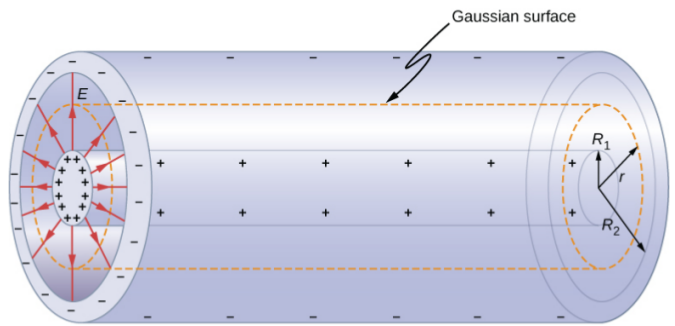
\includegraphics[width=0.7\textwidth]{figures/cyl.png}
\caption{\label{fig:cyl} A cylindrical capacitor, as a model for a coaxial cable.  There is an inner radius and an outer radius, with our Gaussian surface drawn in between the two conductors.}
\end{figure}
\end{frame}

\begin{frame}{The Cylindrical Capacitor and Coaxial Cables}
Recall that
\begin{align}
Q &= \Delta VC \\
\Delta V &= - \int_{R_1}^{R_2} \vec{E} \cdot d\vec{r}
\end{align}
\begin{itemize}
\item What is the electric field $\vec{E}$ of a section of this coaxial cable of length $l$? (\textit{Recall from warm-up.}).
\item What if we integrate from positive charge (inner radius) to negative charge (outer)? \textbf{Observe on board.}
\end{itemize}
\end{frame}

\begin{frame}{The Cylindrical Capacitor and Coaxial Cables}
Thus we have the capacitance per unit length:
\begin{equation}
\boxed{
\frac{C}{l} = \frac{2\pi\epsilon_0}{\ln(R_2/R_1)}
}
\end{equation}
What are the units of $\epsilon_0$?
\begin{itemize}
\item A: F/m$^2$
\item B: F/m
\item C: F/$\ln(m)$
\item D: F
\end{itemize}
\end{frame}

\begin{frame}{The Cylindrical Capacitor and Coaxial Cables}
Thus we have the capacitance per unit length:
\begin{equation}
\boxed{
\frac{C}{l} = \frac{2\pi\epsilon_0}{\ln(R_2/R_1)}
}
\end{equation}
Suppose the cap per unit length is 0.1 nF, and we \textit{square} $R_2/R_1$.  What is the new cap per unit length?
\begin{itemize}
\item A: 0.1 nF
\item B: 0.05 nF
\item C: 0.2 nF
\item D: 0 nF
\end{itemize}
\end{frame}

\begin{frame}{The Cylindrical Capacitor and Coaxial Cables}
Thus we have the capacitance per unit length:
\begin{equation}
\boxed{
\frac{C}{l} = \frac{2\pi\epsilon_0}{\ln(R_2/R_1)}
}
\end{equation}
Suppose the cap per unit length is 0.1 nF, and we \textit{triple} $\epsilon_0$ in some way.  What is the new cap per unit length?
\begin{itemize}
\item A: 0.1 nF
\item B: 0.2 nF
\item C: 0.3 nF
\item D: 0.5 nF
\end{itemize}
\end{frame}

\begin{frame}{The Cylindrical Capacitor and Coaxial Cables}
(Preview of Unit 3).  Suppose we have a system that obeys
\begin{equation}
v(t) = R \frac{dQ}{dt} = i(t) R
\end{equation}
This is called \textbf{Ohm's law.}
\begin{figure}
\centering
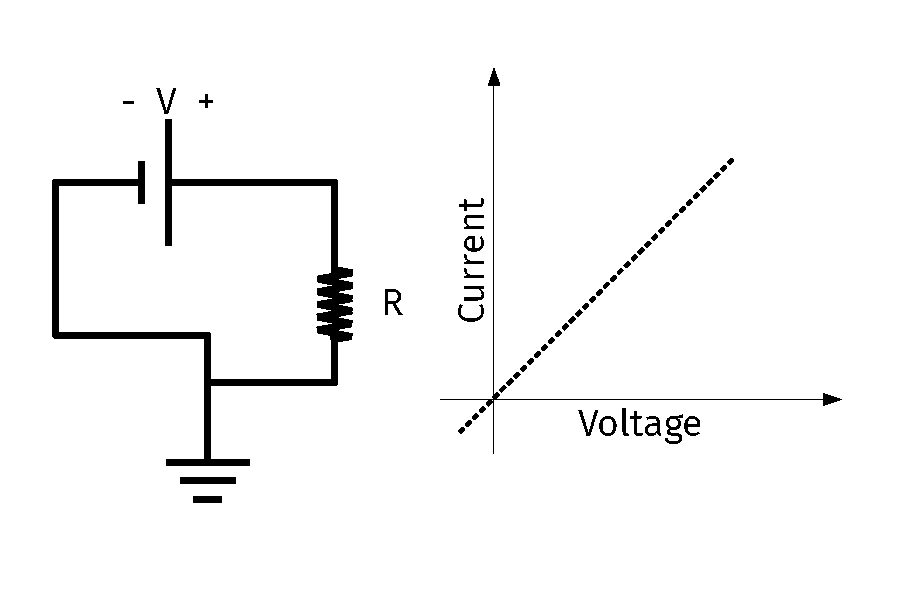
\includegraphics[width=0.55\textwidth]{figures/iVCurve.pdf}
\caption{\label{fig:iv} A simple circuit with a resistor element, some voltage, and \textit{ground.} This just means that 0V is at the negative terminal.}
\end{figure}
\end{frame}

\begin{frame}{The Cylindrical Capacitor and Coaxial Cables}
(Preview of Unit 3).  What if we add a capacitor?
\begin{equation}
V_0 = R \frac{dQ}{dt} +\frac{Q}{C}
\end{equation}
This is called \textbf{Ohm's law.}
\begin{figure}
\centering
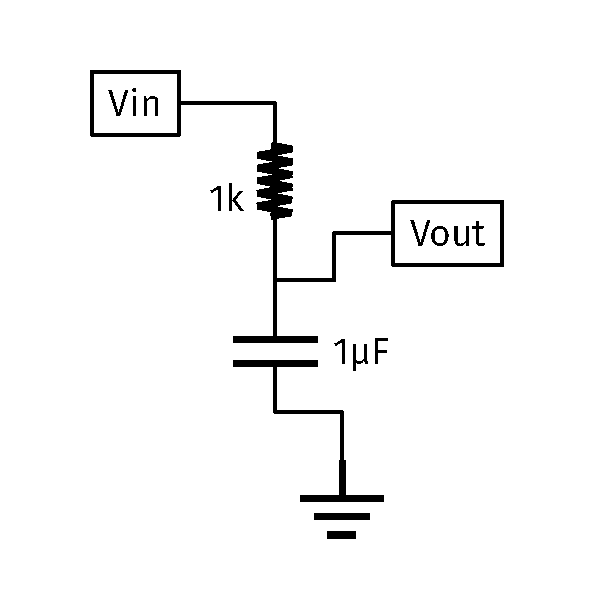
\includegraphics[width=0.45\textwidth]{figures/iVCurve8.pdf}
\caption{\label{fig:iv2} A simple circuit with a resistor and capacitor elements.}
\end{figure}
\end{frame}

\begin{frame}{The Cylindrical Capacitor and Coaxial Cables}
(Preview of Unit 3).  What if we add a capacitor?
We can show that
\begin{equation}
V_{out}(t) = V_0 \exp(-t/\tau)
\end{equation}
with $\tau = RC$.  Thus, if we send a signal $V_{in}$ down a ``very long'' coaxial cable, with some capacitance per unit length, it will not exit the cable. \\ \vspace{0.5cm}
For example: \url{https://www.pasternack.com/images/ProductPDF/LMR-400.pdf} \\ \vspace{0.5cm}
What is the attenuation per 100 m of this cable at 150 MHz?
\end{frame}

\section{Current}

\begin{frame}{Current}
\underline{Notions of current:}
\begin{itemize}
	\item $I = \frac{\Delta Q}{\Delta t}$ - The derivative of charge
	\item The \textit{movement} of electrons
	\item The \textit{flow} of charge
	\item Number of Coulombs per second (1 Amp = C/s)
\end{itemize}
\underline{There is an interesting problem with the notion of current} \underline{as movement of charges.} \\ \vspace{0.5cm}
\begin{columns}[T]
\begin{column}{0.5\textwidth}
Speed of typical electronic signals: $\approx 10^{8}$ m/s
\end{column}
\begin{column}{0.5\textwidth}
Typical speed of actual charges passing through a conductor under voltage: $\approx 10^{-4}$ m/s
\end{column}
\end{columns} \vspace{0.25cm}
\textbf{Since there is a 12 order of magnitude range, it's probably a good idea to ponder...}
\end{frame}

\begin{frame}{Current}
\small
Are the electrons colliding/interacting to form electrical signals?  Or just moving all together?
\begin{figure}
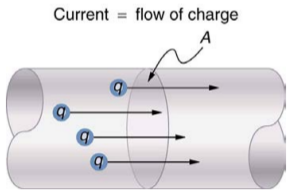
\includegraphics[width=0.5\textwidth]{figures/current1.png}
\caption{\label{fig:current1} The \textit{drift velocity} is the average velocity of an electron, and current is derived from this average velocity.}
\end{figure}
\end{frame}

\begin{frame}{Current}
So we see how electrical signals can move near the speed of light, but we measure the movements of electrons in circuits to be slow.  Can we make a calculation to understand the speed of the electrons? \\ \vspace{0.5cm}
\begin{figure}
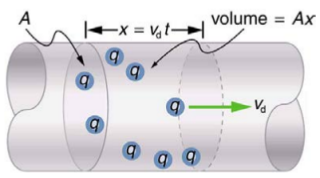
\includegraphics[width=0.5\textwidth]{figures/current3.png}
\caption{\label{fig:current3} Consider the volume $V$ of conductor with cross-sectional area $A$ and length $\Delta x$, having $n$ free electrons per unit volume.}
\end{figure}
\end{frame}

\begin{frame}{Current}
An \textbf{amp} is one \textit{Coulomb} per \textit{second}.  The definition of current is
\begin{equation}
I = \frac{\Delta Q}{\Delta t} = \frac{qnA\Delta x}{\Delta t} = q n A v_{\rm d}
\end{equation}
Solving for drift velocity:
\begin{equation}
v_{\rm d} = \frac{I}{q n A}
\end{equation}
Suppose our conductor is a wire with radius $r$ and $A = \pi r^2$.  Substituting,
\begin{equation}
v_{\rm d} = \frac{I}{\pi q n r^2}
\end{equation}
Remember that $q = 1.6 \times 10^{-19}$ C, and $n$ is the number of free electrons \textit{per atom per unit volume}.  How do we get this number?
\end{frame}

\begin{frame}{Current}
\textbf{Number density}: The total number of objects in a system is equal to the \textit{number density} times the volume of the system.
\begin{equation}
N = nV
\end{equation}
\begin{itemize}
\item N: Total number
\item n: \textit{number density}
\item V: Volume
\end{itemize}
\end{frame}

\begin{frame}{Current}
\textbf{Example:} \alert{Number of Stars in the Milky Way}.  How many stars are in our galaxy?  Assume the galaxy is a disk of height $h$ and radius $r$.  We observe $n$ stars per unit volume.
\begin{itemize}
\item $r$ = $50 \times 10^3$ \textit{light-years}
\item $h = 2 \times 10^3$ \textit{light-years}
\item $n = 10^{-2}$ \textit{light-year} $^{-3}$
\end{itemize}
\begin{enumerate}
\item Compute the volume in \textit{light-years}$^3$
\item Multiply the volume by the number density to obtain the total number.
\item Compare the result with others' results.
\end{enumerate}
\end{frame}

\begin{frame}{Current}
\small
How many \textbf{conduction} electrons are there in a cube of copper that is 1 micron (1 $\mu$m = $10^{-6}$ m) on a side?
\begin{itemize}
\item Copper has a density of 8.8 grams per cubic centimeter.
\item Copper has an atomic weight of 63.54 grams per mole.  (\textit{Do you remember what a mole is?}).
\item There are $N_A = 6.02 \times 10^{23}$ atoms per mole.
\item Only one electron per atom of copper is a conduction electron.
\end{itemize} \hrulefill
\begin{enumerate}
\item Divide the density by the atomic weight.  What are the units?
\item Multiply by $N_A$ (Avogadro's number).  What are the units?
\item Convert the units from $cm^{-3}$ to $\mu m^{-3}$.
\end{enumerate}
\end{frame}

\begin{frame}{Current}
\textbf{Number density}: Let's examine copper, a common wire material with one free electron per atom.  Copper has a density of 8800 kg/m$^3$, and $0.06354$ kg/mol.  There are $6.02 \times 10^{23}$ atoms/mol.  How many free electrons per m$^3$ of copper? (Remember that there is only one conduction electron per copper atom).
\begin{itemize}
\item A: $10^{26}$ free electrons per m$^3$
\item B: $10^{27}$ free electrons per m$^3$
\item C: $10^{28}$ free electrons per m$^3$
\item D: $10^{29}$ free electrons per m$^3$
\end{itemize}
\end{frame}

\begin{frame}{Current}
Consider a copper wire with radius $r = 2.053$ mm that is carrying 20.0 A of current.  Using $q = 1.6\times 10^{19}$, and $n = 8.34 \times 10^{28}$ electrons/m$^3$, and $v_{\rm d} = I/(\pi q n r^2)$, compute the drift velocity of charge in the wire.  \textit{This is a common situation in household wiring.}
\begin{itemize}
\item A: $10^{-1}$ m/s
\item B: $10^{-2}$ m/s
\item C: $10^{-3}$ m/s
\item D: $10^{-4}$ m/s
\end{itemize}
\end{frame}

\begin{frame}{Current}
\textbf{Drift speed vs. signal speed}.  Given that the electrons move at 1 mm/s, how is it that electric signals move at $10^8$ m/s? \\ \vspace{1cm}
\textbf{Electrical signals are \alert{waves} of charge}: \\ \url{https://phet.colorado.edu/en/simulation/legacy/wave-on-a-string}
\end{frame}

\begin{frame}{Current}
\textit{Current as the derivative of charge:} $I = dQ/dt$.  Suppose a bolt of lightning lasts for 0.5 ms, and carries a current of 30 kA (kilo-amps).  How many Coulombs of charge does it deliver?
\begin{itemize}
\item A: 1.5 C
\item B: 15 C
\item C: 150 C
\item D: 1500 C
\end{itemize}
\end{frame}

\begin{frame}{Current}
\textit{Current as the derivative of charge:} $I = dQ/dt$.  Suppose a bolt of lightning lasts for 5 ms, and the current is described by $I(t) = \alpha t$, with $\alpha = 2\times 10^3$ C/s$^2$.  How many Coulombs of charge does it deliver?
\begin{itemize}
\item A: 2.5 C
\item B: 0.25 C
\item C: 0.025 C
\item D: 0.0025 C
\end{itemize}
\end{frame}

\section{Resistivity and Resistance}

\begin{frame}{Resistivity and Resistance}
\textbf{Resistivity} $\rho$ and \textbf{conductivity} $\sigma$ are intrinsic properties of materials, and they are reciprocals of each other:
\begin{equation}
\rho = 1/\sigma
\end{equation}
Let $\vec{J}$ be the \textit{current density}.  The most general form of Ohm's law is
\begin{equation}
\boxed{
\vec{J} = \sigma \vec{E}}
\end{equation}
Let's assume that current is flowing down a conductor of length $L$ and cross-sectional area $\vec{A}$, parallel to $\vec{E}$.  Integrate both sides:
\begin{align}
I &= \sigma \int \vec{E} \cdot \vec{dA} = \sigma E A = \frac{\sigma V}{L} A \\
V &= \frac{L \rho}{A} I = I R
\end{align} 
\end{frame}

\begin{frame}{Resistivity and Resistance}
Thus, the \textit{resistance} of an object is 
\begin{equation}
R = \frac{L \rho}{A}
\end{equation}
The resistivity has units of Ohm meters.  Which of the following is true of a conductor?
\begin{itemize}
\item A: Lengthening it increases the resistance, and widening it increases the resistance.
\item B: Lengthening it decreases the resistance, and widening it increases the resistance.
\item C: Lengthening it increases the resistance, and widening it decreases the resistance.
\item D: Lengthening it decreases the resistance, and widening it decreases the resistance.
\end{itemize}
\end{frame}

\begin{frame}{Resistivity and Resistance}
Thus, the \textit{resistance} of an object is 
\begin{equation}
R = \frac{L \rho}{A}
\end{equation}
Suppose the length of a conductor is doubled, and the area is quadrupled.  By how much does the resistance change?
\begin{itemize}
\item A: It decreases by a factor of two.
\item B: It decreases by a factor of four.
\item C: It increases by a factor of two.
\item D: It increases by a factor of four.
\end{itemize}
\end{frame}

\begin{frame}{Resistivity and Resistance}
What is the resistance of a 1 meter-long wire with area 3 mm$^2$ that made from a metal that has $\rho = 10^{-7}$ $\Omega$ m?
\begin{itemize}
\item A: 0.01 Ohms
\item B: 0.1 Ohms
\item C: 1.0 Ohms
\item D: 10.0 Ohms
\end{itemize}
\end{frame}

\begin{frame}{Resistivity and Resistance}
\begin{figure}
\centering
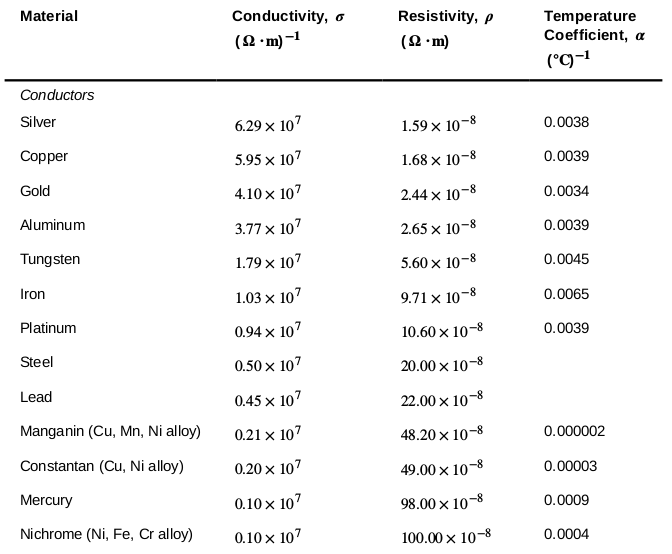
\includegraphics[width=0.8\textwidth]{figures/resist.png}
\caption{\label{fig:resist} Resistivities of various metals.}
\end{figure}
\end{frame}

\begin{frame}{Resistivity and Resistance}
Like the expansion of metals with increasing temperature, \textit{resistivity has a temperature dependence.}  Let $\Delta T = T - T_0$, with $T_0 = 20.0$ C.
\begin{equation}
\rho = \rho_0 \exp \left( \alpha \Delta T \right)
\end{equation}
Using a Taylor series around $\Delta T = 0$, we find
\begin{equation}
\rho(T) \approx \rho_0 \left(1 + \alpha \Delta T \right)
\end{equation}
\end{frame}

\begin{frame}{Resistivity and Resistance}
\begin{figure}
\centering
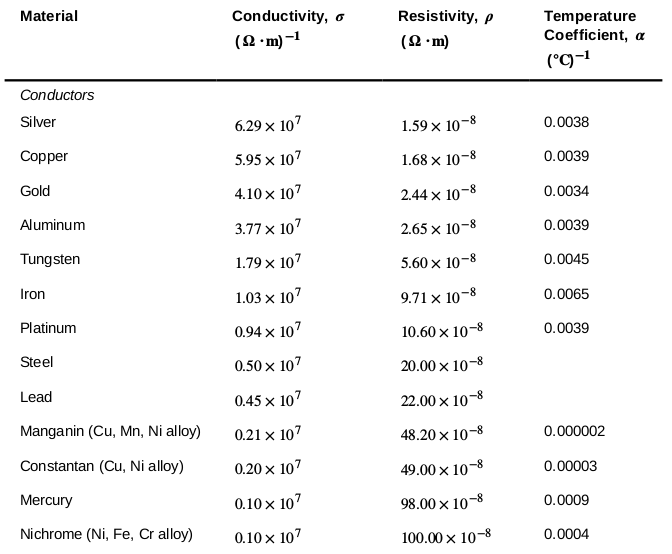
\includegraphics[width=0.7\textwidth]{figures/resist.png}
\caption{\label{fig:resist2} Resistivities of various metals.  Notice the temperature coefficients are small, so the Taylor series is justified.}
\end{figure}
\end{frame}

\begin{frame}{Resistivity and Resistance}
Consider a copper wire that has a resistance of 0.1 Ohms at 20 degrees C.  What will be the resistance of the wire at 40 degrees C, if the temperature coefficient of copper resistivity is 0.004?
\begin{itemize}
\item A: 0.104 Ohms
\item B: 0.108 Ohms
\item C: 0.112 Ohms
\item D: 0.116 Ohms
\end{itemize}
\end{frame}

\begin{frame}{Current}
Consider a copper wire that has a resistance of 5 Ohms at 20 degrees C.  What will be the resistance of the wire at 50 degrees C, if the temperature coefficient of copper resistivity is 0.004?
\begin{itemize}
\item A: 4.8 Ohms
\item B: 5.0 Ohms
\item C: 5.6 Ohms
\item D: 6.0 Ohms
\end{itemize}
\end{frame}

\begin{frame}{Current}
Given that we found a 12\% increase in the resistance of the wire in the prior example, what would happen to the voltage delivered to a device at the other end of that wire?
\begin{itemize}
\item A: It would be unaffected.
\item B: It would decrease by 12 percent.
\item C: It would increase by 12 percent.
\item D: It would decrease by 6 percent.
\end{itemize}
\textit{So you can see why we don't do DC power transmission over long distances.}
\end{frame}

\section{Power}

\begin{frame}{Power}
Notice that if $P = dU/dt$ and $U = qV$, then $P = V dq/dt = IV$, at a constant voltage.
\begin{equation}
P = IV = \frac{I^2}{R}
\end{equation}
\begin{figure}
\centering
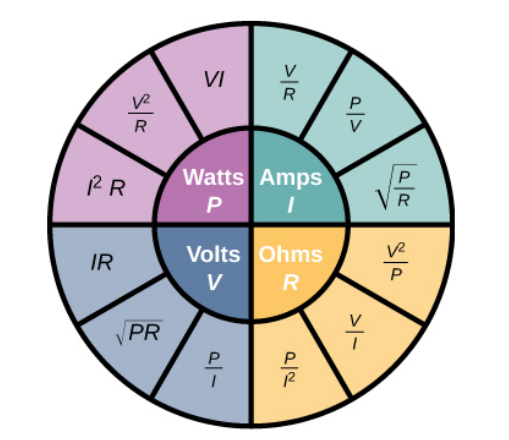
\includegraphics[width=0.33\textwidth]{figures/wheel.png}
\caption{\label{fig:power} The many relationships between electrical quantities in DC circuits.}
\end{figure}
\textbf{Practical example: home energy consumption.} (Example 9.10).
\end{frame}

\section{Batteries and Internal Resistance}

\begin{frame}{Batteries and Internal Resistance}
\small
\begin{enumerate}
\item A battery is a series of electrochemical \textit{cells}.
\item The \textbf{cathode} gives electrons to the \textbf{anode}.
\item Molecular acid-base reactions ``pump'' charge to a higher potential at the cost of some internal resistance.
\end{enumerate}
\begin{figure}
\centering
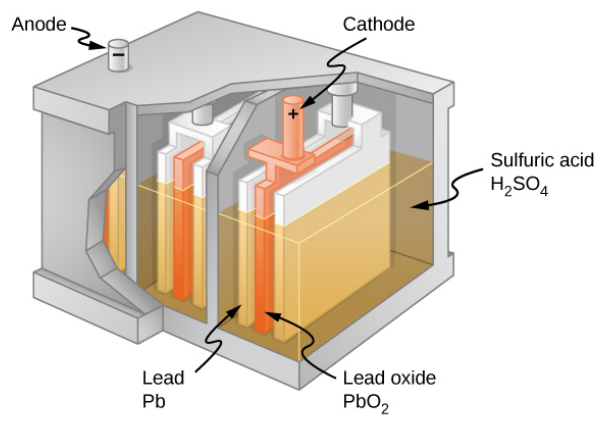
\includegraphics[width=0.5\textwidth]{figures/batt.png}
\caption{\label{fig:batt} A simplified view of a liquid Pb-acid battery.}
\end{figure}
\end{frame}

\begin{frame}{Batteries and Internal Resistance}
\small
\begin{enumerate}
\item A battery is a series of electrochemical \textit{cells}.
\item The \textbf{cathode} gives electrons to the \textbf{anode}.
\item Molecular acid-base reactions ``pump'' charge to a higher potential at the cost of some internal resistance.
\end{enumerate}
\begin{figure}
\centering
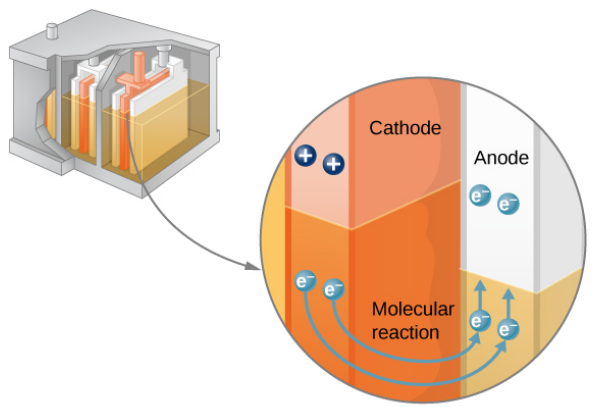
\includegraphics[width=0.5\textwidth]{figures/batt2.png}
\caption{\label{fig:batt2} A microscopic picture of Fig. \ref{fig:batt}.}
\end{figure}
\end{frame}

\begin{frame}{Batteries and Internal Resistance}
\small
\begin{enumerate}
\item The \textit{internal resistance} of a battery obeys the following model.
\item $V_{term} = \epsilon - I r_{int}$
\end{enumerate}
\begin{figure}
\centering
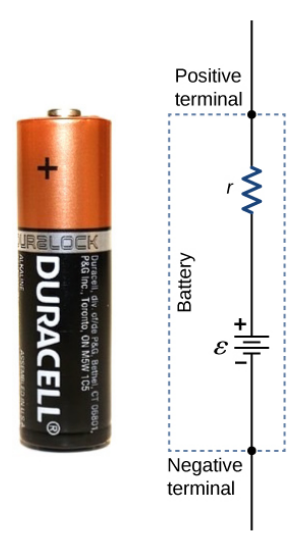
\includegraphics[width=0.25\textwidth]{figures/batt3.png}
\caption{\label{fig:batt3} A good model of battery internal resistance.}
\end{figure}
\end{frame}

\begin{frame}{Batteries and Internal Resistance}
\small
\begin{enumerate}
\item The \textit{internal resistance} of a battery obeys the following model.
\item $V_{term} = \epsilon - I r_{int}$.  A battery may be \textit{rated} at $\epsilon$, but not produce $\epsilon$.
\item To most accurately predict current flow, both $r$ and $R$ must be included (note the labeling of the circuit).
\end{enumerate}
\begin{figure}
\centering
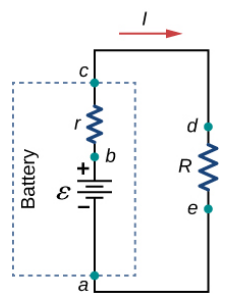
\includegraphics[width=0.25\textwidth]{figures/batt4.png}
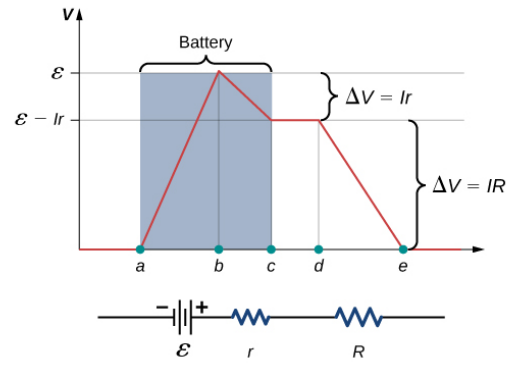
\includegraphics[width=0.5\textwidth]{figures/batt5.png}
\caption{\label{fig:batt4} A good model of battery internal resistance.}
\end{figure}
\end{frame}

\begin{frame}{Batteries and Internal Resistance}
A 5V battery powers a motor with effective resistance of 45 $\Omega$.  If the current draw is 100 mA, what is the internal battery resistance? (\textit{Hint:} draw a diagram and go around the loop).
\begin{itemize}
\item A: 3 $\Omega$
\item B: 30 $\Omega$
\item C: 5 $\Omega$
\item D: 50 $\Omega$
\end{itemize}
\end{frame}

\section{Ohm's Law, Kirchhoff's Rules and Simple Circuits}

\begin{frame}{Ohm's Law, Kirchhoff's Rules and Simple Circuits}
Voltage and capacitance can be combined with another concept, \alert{resistance}, to build an understanding of \alert{circuits}.  Ohm's law is the relationship between \textit{current} and \textit{voltage}:
\begin{equation}
V = I R = \frac{dQ}{dt}R
\end{equation}
Current is the \textit{flow of charge.}  The unit of resistance is called the Ohm, and the unit of current is called the amp, for Amp\`{e}re.
\end{frame}

\begin{frame}{Ohm's Law, Kirchhoff's Rules and Simple Circuits}
A 9 V battery powers a smoke detector, and the current is 0.009 amps.  What is the resistance of the circuit powering the smoke detector?
\begin{itemize}
\item A: 1000 Ohms
\item B: 100 Ohms
\item C: 10 Ohms
\item D: 1 Ohm
\end{itemize}
\end{frame}

\begin{frame}{Ohm's Law, Kirchhoff's Rules and Simple Circuits}
A 3.3 V battery powers a christmas light, and the current is 0.33 amps.  What is the resistance of the circuit powering the smoke detector?
\begin{itemize}
\item A: 1000 Ohms
\item B: 100 Ohms
\item C: 10 Ohms
\item D: 1 Ohm
\end{itemize}
\end{frame}

\begin{frame}{Ohm's Law, Kirchhoff's Rules and Simple Circuits}
Resistors, capacitors, voltages, and current can be combined conceptually to form \alert{\textbf{DC Circuits}} (direct-current).  The following rules govern the interaction of resistors with each other, and capacitors with each other:
\begin{itemize}
\item For resistors \textit{in series}: $R = R_1 + R_2 + R_3 + ...$
\item For resistors \textit{in parallel}: $R^{-1} = R_1^{-1} + R_2^{-1} + R_3^{-1} + ...$
\item For capacitors \textit{in parallel}: $C = C_1 + C_2 + C_3 + ...$
\item For capacitors \textit{in series}: $C^{-1} = C_1^{-1} + C_2^{-1} + C_3^{-1} + ...$
\end{itemize}
\textbf{Observe on board:} difference between in series, and in parallel? (Hint, different voltage for in series, same voltage for in parallel).
\end{frame}

\begin{frame}{Ohm's Law, Kirchhoff's Rules and Simple Circuits}
Kirchhoff's rules:
\begin{enumerate}
\item Summing the voltage in a loop must equal zero ($\vec{E}$-fields are conservative, energy is conserved).
\item Current through a node is conserved (charge is conserved).
\end{enumerate}
\textbf{Observe on board.}
\end{frame}

\begin{frame}{Ohm's Law, Kirchhoff's Rules and Simple Circuits}
Two resistors have 1 k$\Omega$ each (1000 Ohms).  What is the effective resistance if they are added \textit{in parallel}?
\begin{itemize}
\item A: 1000 Ohms
\item B: 500 Ohms
\item C: 2000 Ohms
\item D: 200 Ohms
\end{itemize}
\end{frame}

\begin{frame}{Ohm's Law, Kirchhoff's Rules and Simple Circuits}
Two capacitors have 1 nF each.  What is the effective capacitance if they are added \textit{in series}?
\begin{itemize}
\item A: 0.5 nF
\item B: 5 nF
\item C: 1 nF
\item D: 2 nF
\end{itemize}
\end{frame}

\begin{frame}{Ohm's Law, Kirchhoff's Rules and Simple Circuits}
Two capacitors have 1 nF each.  What is the effective capacitance if they are added \textit{in parallel}?
\begin{itemize}
\item A: 0.5 nF
\item B: 5 nF
\item C: 1 nF
\item D: 2 nF
\end{itemize}
\end{frame}

\begin{frame}{Ohm's Law, Kirchhoff's Rules and Simple Circuits}
\small
\begin{enumerate}
\item Summing the voltage in a loop must equal zero ($\vec{E}$-fields are conservative, energy is conserved).
\item Current through a node is conserved (charge is conserved).
\end{enumerate}
\begin{figure}
\centering
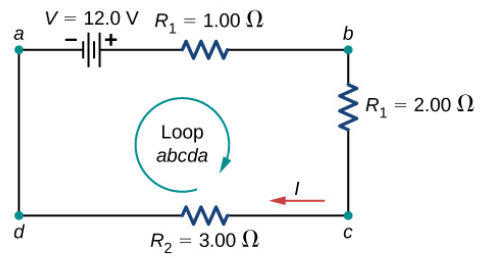
\includegraphics[width=0.5\textwidth]{figures/batt6.png}
\caption{\label{fig:batt5} Using a loop to solve for the current, $I$.  The resistor rule for series resistors comes out of the calculation (observe on board).}
\end{figure}
\end{frame}

\begin{frame}{Ohm's Law, Kirchhoff's Rules and Simple Circuits}
\small
\begin{enumerate}
\item Summing the voltage in a loop must equal zero ($\vec{E}$-fields are conservative, energy is conserved).
\item Current through a node is conserved (charge is conserved).
\end{enumerate}
\begin{figure}
\centering
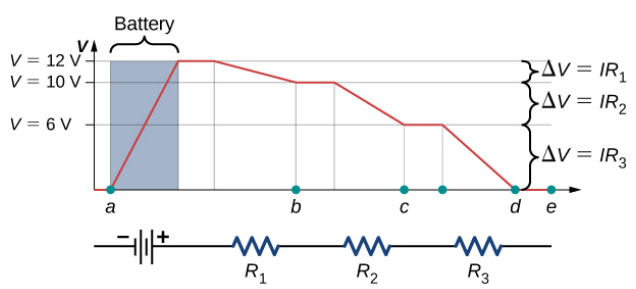
\includegraphics[width=0.5\textwidth]{figures/batt7.png}
\caption{\label{fig:batt6} The result is a complete understanding of voltage and current in the DC circuit.}
\end{figure}
\end{frame}

\begin{frame}{Ohm's Law, Kirchhoff's Rules and Simple Circuits}
\small
\begin{figure}
\centering
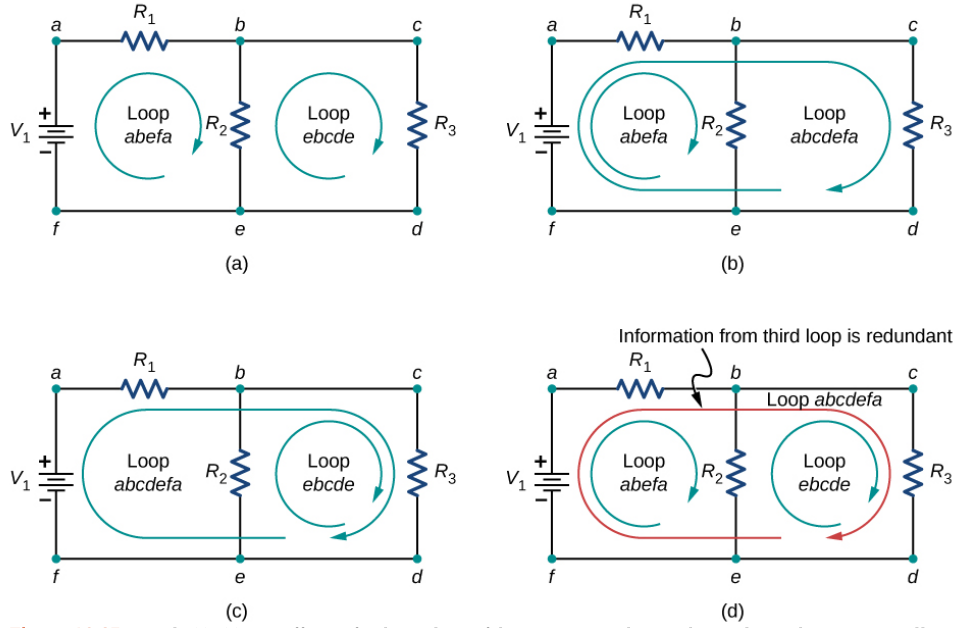
\includegraphics[width=0.75\textwidth]{figures/batt8.png}
\caption{\label{fig:batt7} Loops and nodes produce a \textbf{system of equations}. The number of equations must be equal to the number of unknowns.  \textit{Pay attention to negative/positive signs for voltage and current!}}
\end{figure}
\end{frame}

\begin{frame}{Ohm's Law, Kirchhoff's Rules and Simple Circuits}
\small
\begin{figure}
\centering
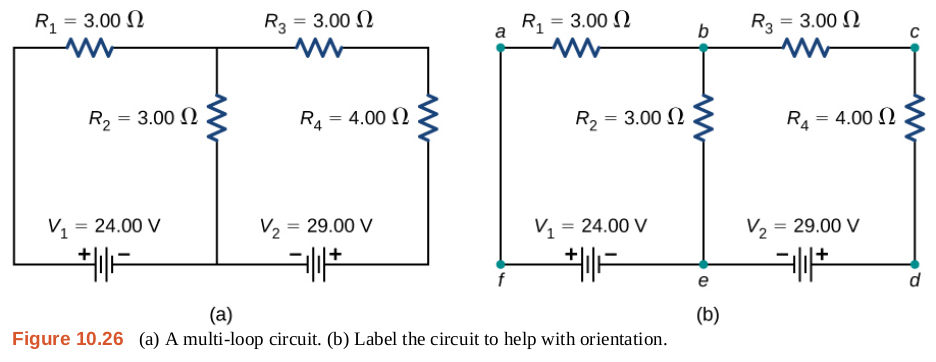
\includegraphics[width=0.9\textwidth]{figures/example1026.png}
\caption{\label{fig:batt8} (1) Label the circuit. (2) Identify nodes with current labels, and loops. (3) Apply Kirchhoff's Rules.}
\end{figure}
\textbf{Work together in groups at tables.} (We'll take this in steps.  First identify two loops and a node...)
\end{frame}

\section{PhET: DC Circuit Modeling}

\begin{frame}{Ohm's Law, Kirchhoff's Rules and Simple Circuits}
\textbf{Use DC circuit PhET simulation to model Fig. \ref{fig:batt8}, checking the currents $I_1$, $I_2$, and $I_3$.} \\ \vspace{1cm}
\url{https://phet.colorado.edu/en/simulation/circuit-construction-kit-dc-virtual-lab} \\ \vspace{1cm}
Do you obtain the same results as the example?  What is the power consumption of this circuit?
\end{frame}

\section{Graphical Analysis of Simple Circuits}

\begin{frame}{Graphical Analysis}
\begin{columns}[T]
\begin{column}{0.5\textwidth}
\begin{figure}
\centering
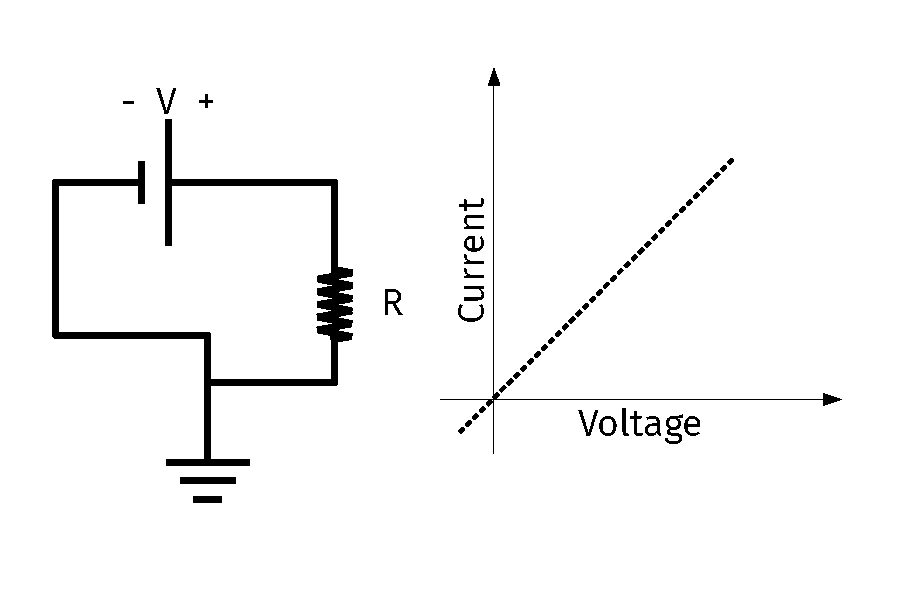
\includegraphics[width=\textwidth,trim=0.5cm 0cm 1cm 0cm,clip=true]{figures/iVCurve.pdf}
\caption{\label{fig:iVCurve1} Circuits components are represented graphically by iV curves.}
\end{figure}
\end{column}
\begin{column}{0.5\textwidth}
\small
If the resistance $R$ is increased, what will happen?
\begin{itemize}
\item A: The slope on the graph will increase
\item B: The slope on the graph will decrease
\item C: The slope will stay the same
\item D: Cannot determine what will happen
\end{itemize}
\end{column}
\end{columns}
\end{frame}

\begin{frame}{Graphical Analysis}
\begin{columns}[T]
\begin{column}{0.5\textwidth}
\begin{figure}
\centering
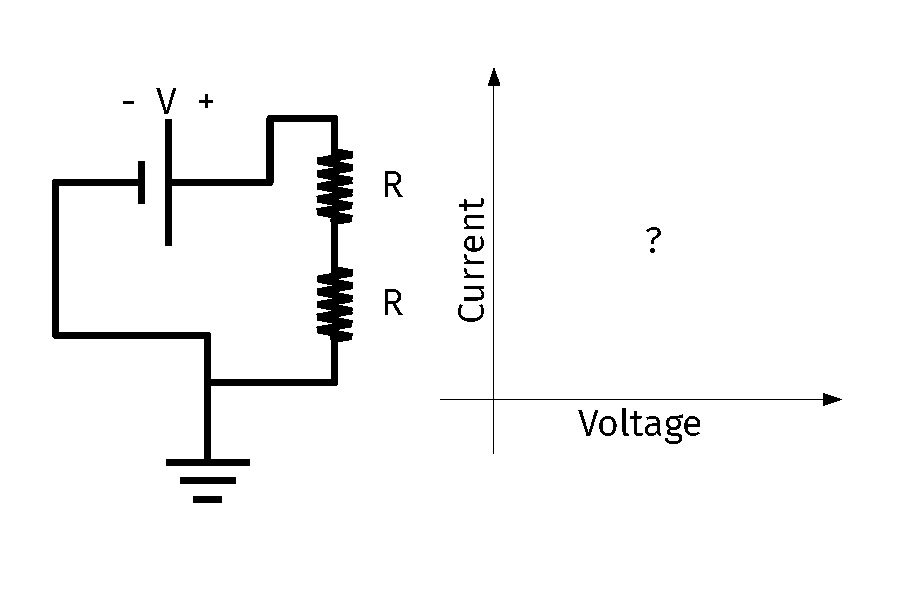
\includegraphics[width=\textwidth,trim=0.5cm 0cm 1cm 0cm,clip=true]{figures/iVCurve2.pdf}
\caption{\label{fig:iVCurve2} Circuits components are represented graphically by iV curves.}
\end{figure}
\end{column}
\begin{column}{0.5\textwidth}
\small
Should the slope now be greater than, less than, or equal to the that of Fig. \ref{fig:iVCurve1}?
\begin{itemize}
\item A: Greater than Fig. \ref{fig:iVCurve1}
\item B: Less than Fig. \ref{fig:iVCurve1}
\item C: Equal to Fig. \ref{fig:iVCurve1}
\item D: Cannot determine.
\end{itemize}
\end{column}
\end{columns}
\end{frame}

\begin{frame}{Graphical Analysis}
\begin{columns}[T]
\begin{column}{0.5\textwidth}
\begin{figure}
\centering
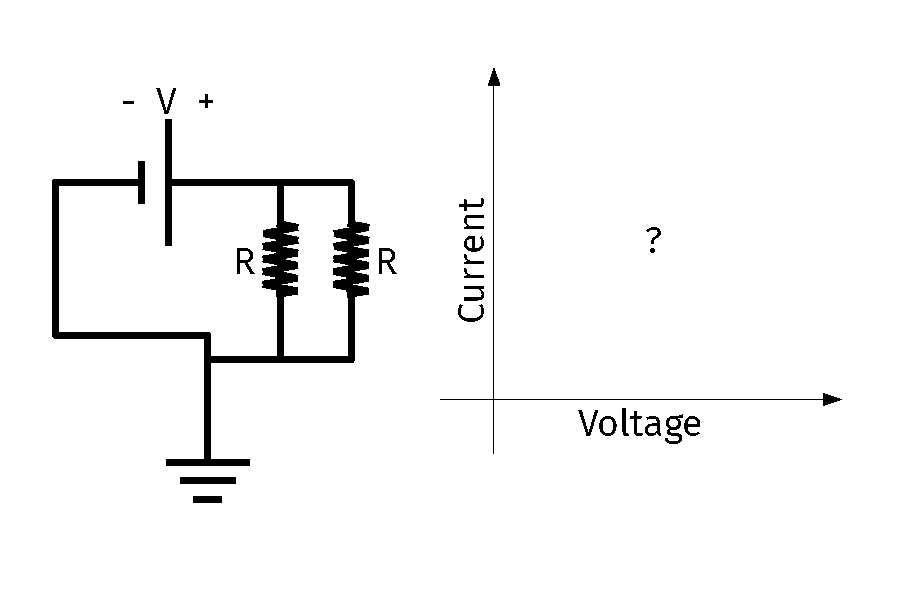
\includegraphics[width=\textwidth,trim=0.5cm 0cm 1cm 0cm,clip=true]{figures/iVCurve3.pdf}
\caption{\label{fig:iVCurve3} Circuits components are represented graphically by iV curves.}
\end{figure}
\end{column}
\begin{column}{0.5\textwidth}
\small
Should the slope now be greater than, less than, or equal to the that of Fig. \ref{fig:iVCurve1}?
\begin{itemize}
\item A: Greater than Fig. \ref{fig:iVCurve1}
\item B: Less than Fig. \ref{fig:iVCurve1}
\item C: Equal to Fig. \ref{fig:iVCurve1}
\item D: Cannot determine.
\end{itemize}
\end{column}
\end{columns}
\end{frame}

\begin{frame}{Graphical Analysis}
\begin{columns}[T]
\begin{column}{0.5\textwidth}
\begin{figure}
\centering
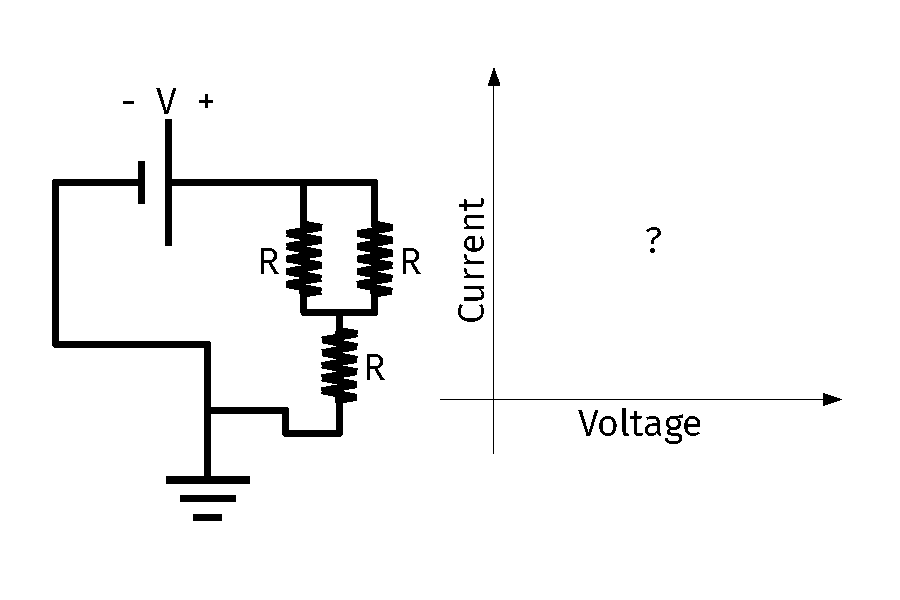
\includegraphics[width=\textwidth,trim=0.5cm 0cm 1cm 0cm,clip=true]{figures/iVCurve4.pdf}
\caption{\label{fig:iVCurve4} Circuits components are represented graphically by iV curves.}
\end{figure}
\end{column}
\begin{column}{0.5\textwidth}
\small
Should the slope now be greater than, less than, or equal to the that of Fig. \ref{fig:iVCurve1}?
\begin{itemize}
\item A: Greater than Fig. \ref{fig:iVCurve1}
\item B: Less than Fig. \ref{fig:iVCurve1}
\item C: Equal to Fig. \ref{fig:iVCurve1}
\item D: Cannot determine.
\end{itemize}
\end{column}
\end{columns}
\end{frame}

\begin{frame}{DC circuit Analysis}
\textbf{Group board exercise:} Solve for the current.
\begin{figure}
\centering
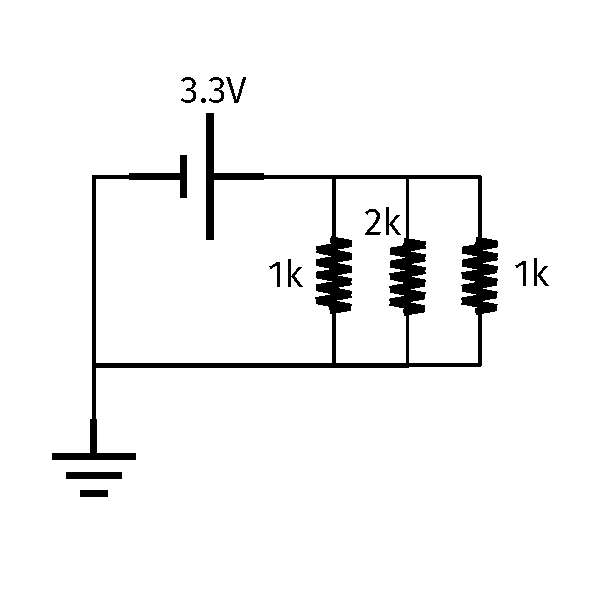
\includegraphics[width=0.5\textwidth]{figures/iVCurve5.pdf}
\caption{\label{fig:iVCurve5} Three resistors in parallel.}
\end{figure}
\end{frame}

\begin{frame}{DC circuit Analysis}
\textbf{Group board exercise:} Solve for the current.
\begin{figure}
\centering
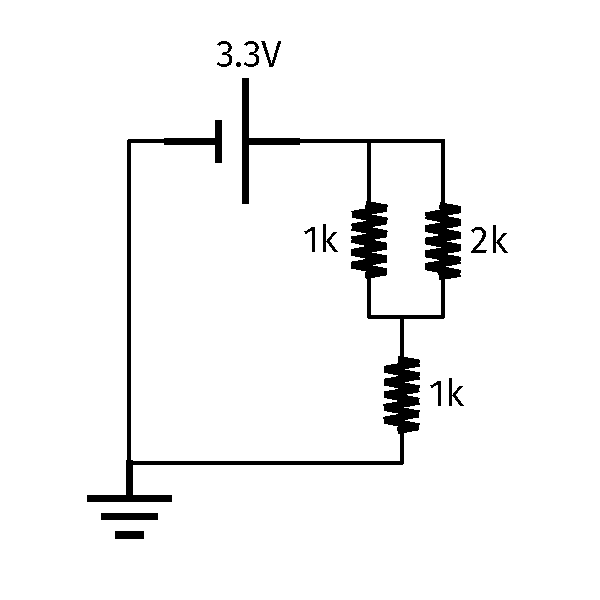
\includegraphics[width=0.5\textwidth]{figures/iVCurve6.pdf}
\caption{\label{fig:iVCurve6} Two resistors in parallel, and in series with a third.}
\end{figure}
\end{frame}

\begin{frame}{DC circuit Analysis}
\textbf{Group board exercise:} Solve for the current.
\begin{figure}
\centering
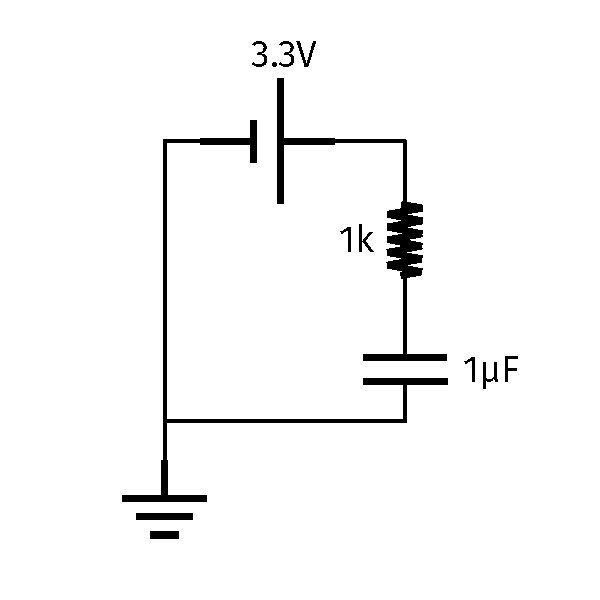
\includegraphics[width=0.5\textwidth]{figures/iVCurve7.pdf}
\caption{\label{fig:iVCurve7} A resistor in series with a capacitor...}
\end{figure}
\end{frame}

\begin{frame}{DC circuit Analysis}
Using Kirchhoff's loop rule:
\begin{align}
V - iR - QC^{-1} &= 0 \\
Q_0 &= CV \\
\tau &= RC \\
\tau \dot{Q} + Q &= Q_0
\end{align}
\textbf{Group board exercise:} Show that the solution for the charge on the capacitor is
\begin{equation}
Q(t) = Q_0 \left(1 - \exp(-t/\tau)\right)
\end{equation}
Take the derivative of both sides to find the current versus time.  Graph the current.
\end{frame}

\begin{frame}{DC circuit Analysis}
So we see that the current is an exponential function:
\begin{equation}
i(t) = i_0 e^{-t/\tau}
\end{equation}
($i_0 = V/R$, the initial current).  What is the current in a circuit with a 1k resistor and a 1 nF capacitor after 3 $\mu$s, if the voltage is 5 V?
\begin{itemize}
\item A: 0.25 mA
\item B: 0.5 mA
\item C: 1.0 mA
\item D: 2.0 mA
\end{itemize}
\end{frame}

\begin{frame}{DC circuit Analysis}
So we see that the current is an exponential function:
\begin{equation}
i(t) = i_0 e^{-t/\tau}
\end{equation}
($i_0 = V/R$, the initial current).  Thinking of the same circuit: when is the current 0.0 mA?
\begin{itemize}
\item A: 3 microseconds
\item B: 30 microseconds
\item C: 300 microseconds
\item D: never
\end{itemize}
\end{frame}

\section{Conclusion}



\section{Answers}

\begin{frame}{Answers}
\small
\begin{columns}[T]
\begin{column}{0.5\textwidth}
\begin{itemize}
\item 2.5V
\end{itemize}
\end{column}
\begin{column}{0.5\textwidth}
\begin{itemize}
\item ..
\end{itemize}
\end{column}
\end{columns}
\end{frame}

\end{document}
